% ============================================================================
% PAQ-KV — supplementary material for paq_aaai_v3.tex (extracted 2026-07-26
% from that file's appendix; every number verbatim, nothing re-derived).
% Cross-document referencing convention: plain numbers (\S4.2, Table 1,
% Figure 3) refer to the MAIN paper and are STATIC TEXT here (update by hand
% if the main paper renumbers); floats in THIS document are numbered S1, S2,
% ... via \thetable/\thefigure/\thealgorithm renewals. The main paper's
% 'Suppl. \S X / Table SX' pointers are likewise static; keep the two
% documents' structures in sync (mapping in the main file's header).
% 2026-07-29 (page-limit pass, mirroring the main paper): fig:sealed moved
% in from main \S5.2 -> A.2 (= Figure S1; old figures shift to S2/S3) and
% main Table 2 (tab:systems) + full \S5.4 prose moved in -> NEW subsection
% C.6 app:systems (= Table S10, at the END of section C so S1-S9 and all
% subsection numbers stay put). Every number verbatim; nothing re-derived.
% Build: ./tectonic -X compile paq_aaai_v3_supplement.tex
% ============================================================================
\documentclass[letterpaper]{article} % DO NOT CHANGE THIS
% ---------------------------------------------------------------------------
% LOCAL BUILD SHIM (this block only; the style file itself is untouched):
% the host has no pdflatex, so this draft is built with tectonic (XeTeX-based).
% aaai2027.sty's engine guard (\RequirePDFTeX) is neutralized ONLY when the
% engine is not pdfTeX. Under the official pdflatex build this block is inert
% and the guard runs as shipped. Remove the shim for the actual submission.
\usepackage{iftex}
\ifPDFTeX\else\let\RequirePDFTeX\relax\fi
% ---------------------------------------------------------------------------
\usepackage[submission]{aaai2027}  % DO NOT CHANGE THIS
\usepackage[hyphens]{url}  % DO NOT CHANGE THIS
\usepackage{graphicx} % DO NOT CHANGE THIS
\urlstyle{rm} % DO NOT CHANGE THIS
\def\UrlFont{\rm}  % DO NOT CHANGE THIS
\usepackage{natbib}  % DO NOT CHANGE THIS AND DO NOT ADD ANY OPTIONS TO IT
\usepackage{caption} % DO NOT CHANGE THIS AND DO NOT ADD ANY OPTIONS TO IT
\frenchspacing  % DO NOT CHANGE THIS
\usepackage{algorithm}
\usepackage{algorithmic}
\usepackage{booktabs}
\usepackage{multirow}
\usepackage{amsmath}
\usepackage{amssymb}


\pdfinfo{
/TemplateVersion (2027.1)
}

\setcounter{secnumdepth}{2}

\graphicspath{{figures/}}

\newcommand{\paq}{\textsc{PAQ}}
\newcommand{\paqt}{\textsc{PAQ-T}}
\newcommand{\paqc}{\textsc{PAQ-KV}}
\newcommand{\lb}{\mathrm{LB}_{95}}
% Below-page isolation-gate numbers, generated by BASED/scripts/paq_isogate_tex.py from
% research/paq_isogate_kv_verdict.json (2026-07-26 run; nothing hand-entered).
% GENERATED by scripts/paq_isogate_tex.py 2026-07-26 10:54 — DO NOT EDIT BY HAND
% source: research/paq_isogate_kv_verdict.json (pin research/paq_confirm_pin.json sha 01f4e203ec67c2d5; n_complete=907/907; verdict=REVERSIBILITY_ISOLATED_BELOWPAGE)

\newcommand{\isoKVLduCommitDelta}{+0.211}
\newcommand{\isoKVLduCommitLb}{+0.136}
\newcommand{\isoKVLduCommitUb}{+0.289}
\newcommand{\isoKVLduCommitCI}{[+0.136,+0.289]}
\newcommand{\isoKVLduStaticDelta}{+0.230}
\newcommand{\isoKVLduStaticLb}{+0.178}
\newcommand{\isoKVLduStaticUb}{+0.276}
\newcommand{\isoKVLduStaticCI}{[+0.178,+0.276]}
\newcommand{\isoKVLduFresh}{0.531}
\newcommand{\isoKVLduCommitAcc}{0.320}
\newcommand{\isoKVLduStaticAcc}{0.301}
\newcommand{\isoKVLduNc}{463}
\newcommand{\isoKVLduNdocs}{80}
\newcommand{\isoKVMmCommitDelta}{+0.137}
\newcommand{\isoKVMmCommitLb}{+0.103}
\newcommand{\isoKVMmCommitUb}{+0.169}
\newcommand{\isoKVMmCommitCI}{[+0.103,+0.169]}
\newcommand{\isoKVMmStaticDelta}{+0.213}
\newcommand{\isoKVMmStaticLb}{+0.160}
\newcommand{\isoKVMmStaticUb}{+0.266}
\newcommand{\isoKVMmStaticCI}{[+0.160,+0.266]}
\newcommand{\isoKVMmFresh}{0.405}
\newcommand{\isoKVMmCommitAcc}{0.268}
\newcommand{\isoKVMmStaticAcc}{0.192}
\newcommand{\isoKVMmNc}{444}
\newcommand{\isoKVMmNdocs}{80}
\newcommand{\isoKVPoolCommitDelta}{+0.174}
\newcommand{\isoKVPoolCommitLb}{+0.132}
\newcommand{\isoKVPoolCommitCI}{[+0.132,+0.215]}
\newcommand{\isoKVPoolStaticDelta}{+0.221}
\newcommand{\isoKVPoolStaticLb}{+0.184}
\newcommand{\isoKVPoolStaticCI}{[+0.184,+0.256]}
\newcommand{\isoKVNComplete}{907}
\newcommand{\isoKVNPinned}{907}
\newcommand{\isoKVNIncomplete}{0}
\newcommand{\isoKVVerdict}{met}


\newcommand{\jiahui}[1]{\textcolor{red}{[Jiahui: #1]}}

\title{PAQ-KV: Supplementary Material}
\author{
    Anonymous submission
}
\affiliations{
    Anonymous submission
}

\renewcommand{\thetable}{S\arabic{table}}
\renewcommand{\thefigure}{S\arabic{figure}}
\makeatletter\@addtoreset{algorithm}{section}\makeatother
\renewcommand{\thealgorithm}{S\arabic{algorithm}}

\begin{document}

\maketitle

\noindent This document provides the supplementary material for the
submission ``Prefill Once, Ask Many: Training-Free Reversible Below-Page KV
Selection for Multi-Query Long-Document Visual Question Answering''
(\paqc{}). Plain-numbered references (\S4.2, Table~1, Figure~3) point to
the main paper; floats in this document are numbered S1, S2, \ldots
Notation follows the main paper: MMLB abbreviates MMLongBench-Doc, LDU
abbreviates LongDocURL, paired contrasts are reported as $\Delta$ $[l,u]$
with document-clustered bootstrap 95\% confidence intervals, and $\lb$ is
the interval's lower bound.

\appendix


% ============================================================================
% Appendix reorganized 2026-07-26 into four thematic sections (AAAI framing
% pass): A implementation/reproducibility, B complete results, C additional
% analyses, D limitations detail. All previous labels are preserved on the
% subsections; material moved out of the main body (integrity narratives,
% mechanism checks, negative results, cross-reader table, contrast table)
% lands here verbatim. This appendix will later become the separate
% supplementary document.
% ============================================================================

\section{Implementation and Reproducibility}\label{app:impl}

\subsection{Pin Construction, Algorithm, and Gate Materials}\label{app:method-materials}

\paragraph{Pin construction.} For each document we build the union of the
benchmark's own-document pages across that document's queries, dropping
cross-document 64K padding, so every query's evidence is present in one
prefill. Documents qualify with at least three gold-bearing queries and at
most 110 union pages, a bound that targets the nominal ${\approx}64$K-token
context at read resolution (realized lengths reach ${\approx}92$K on the
largest documents); selection is seed-0 frozen. Table~\ref{tab:pins}
summarizes the confirmatory pin.

\begin{algorithm}[t]
\caption{\paqc{}: per-query reversible below-page KV-block selection with a 4D restricted-attention mask}
\label{alg:paqc}
\begin{algorithmic}[1]
\REQUIRE document pages rendered as in the full-context arm ($\le$64K tokens); queries $q_1,\ldots,q_k$; nominal budget $b=5\%$; frozen VLM
\STATE prefill the document once; retain the full KV cache $C$ (context length $n_{\mathrm{ctx}}$); record page-aligned 64-token block spans $B_1,\ldots,B_m$ and the always-keep scaffold set $\mathcal{A}$
\FOR{each query $q_j$}
\STATE forward the tokenized question over $C$; capture question-to-context attention via per-layer hooks; \textbf{crop} $C$ back to $n_{\mathrm{ctx}}$
\STATE $\mathrm{score}(B_i) \gets$ aggregated question-row attention mass on block $B_i$'s positions
\STATE $S_j \gets$ top blocks by score at the nominal budget $b \cdot n_{\mathrm{ctx}}$
\STATE build the 4D additive mask $M_j$: decode rows may attend to $\mathcal{A} \cup S_j \cup q_j \cup{}$generated tokens; all other context positions get $-\infty$
\STATE decode the answer from $C$ under $M_j$; no gathering, so K/V positions and M-RoPE indices are unchanged
\STATE discard $M_j$; $C$ is intact for $q_{j+1}$
\ENDFOR
\end{algorithmic}
\end{algorithm}

\begin{table}[t]
\centering\small
\setlength{\tabcolsep}{4pt}% permitted narrowing (AAAI kit)
\begin{tabular}{lcc}
\toprule
 & LDU & MMLB \\
\midrule
Documents & 80 & 80 \\
Complete queries at gate & 463 & 444 \\
Gold-bearing queries / doc & 5.79 & 5.50 \\
Median (mean) union pages & 44 (45.0) & 28 (36.5) \\
\bottomrule
\end{tabular}
\caption{The confirmatory evaluation pin. ``Complete queries'' are rows where every gated arm scored; the below-page gate completed all 907 pinned queries with zero skips, so no imputation was needed (the historical page-level run had 4 timeout-missing queries, immaterial under worst-case imputation).}
\label{tab:pins}
\end{table}

% Environment facts verified 2026-07-29 against the frozen-meta JSONs
% (do_sample/max_new_tokens/python path) and the `ml` conda env itself
% (torch/transformers/peft/CUDA/GPU); dtype from BASED/scripts/paq.py.
% Deliberately NOT a numbered float: a new table before tab:contrasts would
% shift every static "Table SX" pointer in the main paper.
\paragraph{Hardware and software.} All experiments ran on a single NVIDIA
RTX PRO 6000 Blackwell GPU (96\,GB) under Ubuntu 22.04, with Python 3.11.6,
PyTorch 2.10.0 (CUDA 12.8), \texttt{transformers} 5.5.4, and \texttt{peft}
0.19.1. Models load in bfloat16, and the resolved revision hash of every
model checkpoint is recorded in the released provenance manifests
(\S\ref{app:repro}).

\paragraph{Hyperparameters.} Every setting was frozen before the gate that
uses it; the only tuned selection in the study is the pre-registered,
development-only InternVL tuning study of \S\ref{app:crossreader-table}.
\begin{itemize}\setlength{\itemsep}{.1em}
\item Nominal evidence budget $b=5\%$, the pre-registered gate value; swept
at $\{2.5, 10\}\%$ on the full pin (Table~\ref{tab:budget-sweep}) and at
$\{5,10,20,30\}\%$ in the InternVL tuning study.
\item KV block size $64$ tokens, page-aligned: fixed a priori, no sweep; the
page-granularity comparison of \S\ref{app:mechanism} probes the coarser
limit.
\item Block scorer: mean attention over all layers, heads, and question rows
(Equation~1 of the main paper). Alternatives evaluated and not adopted: max
aggregation (Table~\ref{tab:panel}), a single sharp expert head, and a
learned per-head mixture (\S\ref{app:negatives}).
\item Commit-once aggregate $M=\min(3,k)$ first queries: fixed a priori;
sensitivity checks remain open (\S\ref{app:limitations-detail}).
\item Context target ${\approx}64$K tokens nominal (realized up to
${\approx}92$K) and page rendering at 144\,DPI, both fixed by the pin
protocol above.
\item Decoding: greedy (\texttt{do\_sample=False}),
\texttt{max\_new\_tokens} $=128$, identical across all arms.
\item Attention implementation: SDPA for prefill and decode; eager attention
only during the per-query preview, so question-to-context attention can be
captured by hooks.
\item Seeds: $0$ for pin selection, the random-selection arms, and the
bootstrap; the bootstrap uses $10{,}000$ document-clustered percentile
draws.
\end{itemize}

\subsection{Reproducibility and Protocol Notes}\label{app:repro}

\paragraph{Pre-registration discipline.} Every gate in this study was frozen (bars, comparators, budgets, imputation policy) before its run: the two-comparator isolation gate; the \paqt{} accuracy-evaluation bars (non-inferiority/improvement/inferior margins, per-cell power floors, adversarial missingness imputation); the per-head-mixture transfer gate; and the \paqc{} decode-identity kill criterion, screen gates, per-cell improvement bars, and sharp-scorer (V1) gate. Two early positives did not survive adversarial review and were retracted before this draft: a first isolation gate against the eviction family (invalidated by a weak-static artifact and replaced by the two-comparator gate), and an early ``outperforms the gold-page oracle'' claim (corrected to ``matches'' at power). The commitment-pressure mechanism hypothesis failed its formal test and is reported as exploratory.

\paragraph{Instrumentation.} All significance statements use one instrument: the document-cluster paired bootstrap (10{,}000 draws, seed 0, percentile intervals; equal-cell pooling), unit-tested alongside the gate and pairing logic. Evaluation pins are sha-256 checksummed and byte-verified before use; the screen pin is a strict prefix of the confirmatory pin, and independent-extension analyses use the 50 new documents per cell only. Figures are generated from the verdict artifacts by a single script; nothing is hand-entered. Per-query, per-arm rows, frozen-bar metadata, verdict files, and the adversarial review trail are retained and will be released with the code. The descriptive re-slices in Appendix~\ref{app:anatomy}, the realized-budget figures, the amortized-latency column of Table~\ref{tab:systems}, and the budget sweep of Appendix~\ref{app:budget-sweep} are additional reuses of the development pin and carry no pre-frozen bars.

% Figure source: BASED/research/paq_sealed_final_sealed_verdict.json via
% BASED/scripts/paq_fig_sealed_bar.py (nothing hand-entered). Moved here from
% the main paper (2026-07-29 page-limit pass); referenced there as
% "Supplementary Figure S1".
\begin{figure}[t]
\centering
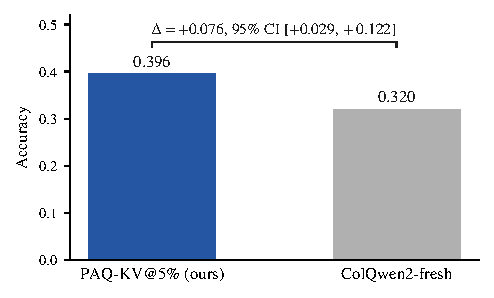
\includegraphics[width=0.92\columnwidth]{figures/fig_sealed_bar.pdf}
\caption{The sealed out-of-sample confirmation on MMLB: accuracy
of \paqc{}@5\% and ColQwen2-fresh on the fresh, disjoint 45-document,
244-query set, evaluated exactly once under the frozen harness (\S4.4 of
the main paper). The bracket reports the paired difference with its
document-clustered bootstrap 95\% CI; only this comparison was run on the
sealed set.}
\label{fig:sealed}
\end{figure}

\paragraph{Sealed-test protocol.} The 80-document confirmatory pin has been reused across this study and is therefore development-only. The fresh sealed set (zero overlap with the pin; 45 MMLB documents / 244 queries, plus 73 LDU documents left unevaluated as out of scope) was evaluated \emph{exactly once} under a guarded, frozen harness: the confirmatory bar (complete-case document-clustered CI lower bound $>0$, with an adversarial worst-case-imputation fallback binding only under any missingness), the corrected-loader comparator, the 5\% budget, the seed, and sha-256 hashes of all eight code components plus the sealed pin were frozen before the run; the harness refuses the sealed pin absent an explicit authorization flag and a typed confirmation, aborts on any component-hash mismatch, and runs a blind non-scoring preflight that can abort without consuming the test. The single run produced the strongest claim in this paper: \paqc{}@5\% $0.396$ vs.\ ColQwen2-fresh $0.320$, $+0.076$ $[+0.029,+0.122]$ ($244/244$ complete, zero skips, robust to adversarial imputation; \S5.2; Figure~\ref{fig:sealed}). The verdict, per-query rows, and a provenance manifest (pin and component hashes, resolved model revisions) are retained and released with the code.

\paragraph{Extended-benchmark overlap audit.} The two added corpora are
corpus-adjacent to ours: MMDocIR was sourced from existing DocVQA collections
including MMLB, and MMDocRAG was built over the MMDocIR document
pool. A document-name audit against our pins found substantial overlap,
including, name for name, the entire sealed MMLB cell inside
MMDocIR's pool. Every document overlapping either the development or the
sealed pins was excluded from the new pins before any experiment ran, so the
sealed reserve remains untouched at the document level; only document names
were read from the sealed pin file, and the audit artifact is retained. The
MMDocRAG pin's protocol deviations are disclosed here: 62 qualifying
documents is below the study's 80-document floor; queries are capped at 12
per document by seed-0 sampling (585 of 1{,}160 kept), a cap the main pins
never needed; pages render at 144\,DPI, matching the existing pins' pixel
scale; gold pages are the union of page identifiers over each query's gold
quotes, with the 0-based convention verified by text-fragment matching on 32
of 32 probes; and answers are scored by the study's shared document-VQA
evaluator. Because 28 of the 62 documents hit the twelve-query cap, we also
decoded the 575 uncapped remainder queries on the same documents: the
\paqc{}-versus-ColQwen2 contrast is $+0.035$ $[+0.019,+0.060]$ on the
remainder and $+0.046$ $[+0.032,+0.064]$ pooled, so the capped cell did not
manufacture the result. The MMDocIR-QA cell reuses the MMDocIR
selection-quality pin and scores against the benchmark's reference answers
with the same shared evaluator. The extended cells reuse the study's frozen
primitives (prefill, preview, selection, decode, the corrected ColQwen2
loader, the shared scorer, and the document-cluster paired bootstrap) but
froze no bars, ran each cell once, and constructed the pins on the day of
the runs. Two follow-ups closed this audit trail. A sealed-style MMDocRAG
reserve was investigated and is structurally empty: none of the 41 remaining
fresh documents qualify under the pin protocol (30 exceed the page ceiling,
11 lack three gold-bearing queries), so the MMDocIR-QA cell of
\S5.3 serves as the independent corroboration lane
instead. And a training-distribution audit of ColQwen2, from its published
training mixture, found no confirmed document-level overlap with any of the
four evaluation corpora; MMDocIR's training split provably shares source
datasets with ColQwen2's mixture, but our cells draw only on its evaluation
pool, and web-crawled slices are unverifiable in both directions, so we
claim neither contamination nor proven disjointness.

\subsection{Methods-Integrity Detail}\label{app:integrity}

This section expands the summary of \S4.4.

\paragraph{Per-query cache pollution.} An independent code review found a
real bug in the per-query scoring loop used across this study: the runtime
mutates the retained cache in place, and the loop reused the document prefill
across a document's queries without restoring it, so query $q_i$ scored while
attending to $q_0\ldots q_{i-1}$. The fix, cropping the cache after every
per-query preview, is now applied everywhere, and its impact was quantified
rather than assumed. On a 24-document, 150-query clean-versus-polluted
re-run, the key isolation contrast is $+0.264$ clean versus $+0.284$
polluted, since the contrast largely cancels the bug when both arms share the
same scorer. Every gate and headline number in this paper postdates the fix,
including the confirmatory isolation gate of \S5.1,
which was re-executed in full on post-fix code with \paqc{} as the fresh arm
and verified at runtime (cache-length assertions after every preview and
decode, plus an order-invariance probe per cell that recomputes a query's
preview after all other queries and requires bit-identity). The one
surviving pre-fix artifact is the historical page-level panel of
Appendix~\ref{app:panel}, whose absolute fresh-arm accuracy carries
${\approx}0.04$ inflation; it is labelled as historical and no claim rests
on its absolute levels. Appendix~\ref{app:reversibility} quantifies the
pollution mechanism itself.

\paragraph{Baseline-loader integrity.} A second independent review caught a
defect in the \emph{comparator}, not in our method: the cached ColQwen2
baseline had run with its trained final retrieval-projection LoRA
(\texttt{custom\_text\_proj}) silently zeroed. \texttt{vidore/colqwen2-v1.0}
is a PEFT adapter, and under our peft/transformers versions a key remap
inserted \texttt{language\_model} into the LoRA target path. The remap is
correct for the language-model layers but wrong for the top-level
\texttt{custom\_text\_proj}, so the checkpoint's projection-LoRA tensors
landed at a non-matching path and the final projection ran with base weights
only. Because the other adapter layers still loaded, the baseline stayed
functional and well above random, which masked the defect until we inspected
the load report and the projection weights directly. We patched the loader,
added a post-load assertion that the two \texttt{custom\_text\_proj} tensors
match the checkpoint, and re-scored ColQwen2. The correction is immaterial to
the main result. Fixed-versus-broken gold-page recall at the 5\% budget is
$0.539$ versus $0.534$. The top-5\% page selections overlap at Jaccard
$0.947$, with only $34$ of $444$ queries changing any selected page.
Re-reading those changed queries moves fresh-read accuracy by $-0.0002$
($0.3282$ corrected versus $0.3284$ broken), and the improvement over
ColQwen2 is $+0.077$ against both loaders ($\lb$ $+0.040$
corrected, $+0.039$ broken), so the main result is not loader-inflated.
The corrected loader is used for the main MMLB comparison
(development and sealed), the MMDocRAG cell, the systems measurement, and,
as of the same-protocol LDU close-out, the LDU comparison as
well (top-5\% selections overlap at Jaccard $0.968$; 25 of 463 queries
changed selection and were re-read; the comparator moves from $0.5124$ to
$0.5121$ and the contrast is $+0.019$ against both loaders, so the
correction is immaterial there too). Only the historical page-level cohort
ever ran with the earlier loader; its panel table
(Appendix~\ref{app:panel}) omits those retrieval rows, and the page-level
narrative of Appendix~\ref{app:pagelevel} quotes them with disclosure.

\section{Complete Experimental Results}\label{app:results}

\subsection{Key Paired Contrasts}\label{app:contrasts}

Table~\ref{tab:contrasts} reports the paired contrasts summarized in
Figure~3b.

\begin{table*}[t]
\centering\scriptsize
\setlength{\tabcolsep}{3pt}
\begin{tabular}{lcccc}
\toprule
 & \multicolumn{3}{c}{$\Delta$ [95\% CI], \paqc{} minus} & \\
\cmidrule(lr){2-4}
Benchmark & ColQwen2-fresh & full-context & gold-page oracle & Bar \\
\midrule
LDU & $+0.019\,[-0.019,+0.061]$ & $-0.014\,[-0.031,+0.003]$ & $-0.078\,[-0.116,-0.040]$ & \textsc{not met} \\
MMLB & $+0.077\,[+0.040,+0.115]$ & $+0.009\,[-0.022,+0.040]$ & $-0.026\,[-0.059,+0.008]$ & \textbf{\textsc{met}} \\
MMLB (sealed) & $+0.076\,[+0.029,+0.122]$ & -- & -- & \textbf{\textsc{met}} \\
MMDocRAG & $+0.057\,[+0.040,+0.076]$ & $+0.007\,[-0.004,+0.018]$ & $+0.006\,[-0.009,+0.022]$ & none frozen \\
MMDocIR-QA & $-0.043\,[-0.065,-0.011]$ & $-0.013\,[-0.049,+0.012]$ & $-0.095\,[-0.158,-0.022]$ & none frozen \\
\bottomrule
\end{tabular}
\caption{Key paired contrasts for Table~1: mean paired
difference $\Delta$ with its document-clustered bootstrap 95\% confidence
interval (10{,}000 draws; \S4.2). The pre-registered
per-cell bar (final column) passes when the CI lower bound of the
ColQwen2-fresh contrast exceeds zero; dashes denote arms not run on the
sealed set. On LDU \paqc{} is below full context, with an interval
that includes zero, and below the gold-page oracle, with an interval that
excludes zero; on MMLB and MMDocRAG it is statistically
indistinguishable from both references. On MMDocIR-QA the trained retriever
significantly outperforms \paqc{}, which remains indistinguishable from its
own full-context read; \S5.3 interprets the
four-cell pattern. The MMDocRAG and MMDocIR-QA cells are development-grade,
so no bars were frozen there.}
\label{tab:contrasts}
\end{table*}

\subsection{Notes on Table~1}\label{app:table1-notes}

SnapKV-fresh scores pages from the same full-resolution prefill \paqc{}
uses, which roughly doubles it over the historical coarse-preview panel of
Appendix~\ref{app:panel}; we treat the same-cohort form as the fair one.
BM25 text channels differ by corpus: LDU has no born-digital text
layer, so its cell uses a tesseract OCR channel (98.1\% of pages recovered),
the MMDocIR-QA cell uses the benchmark's own OCR text field (99.5\%
coverage), and the other cells use born-digital text. The LDU
ColQwen2 cell uses the corrected loader (\S4.4).
MMLB decodes 444 queries; paired contrasts use the 440 with
cached references (the 4 \texttt{mi\_phone} rows lack cached references).
Realized budgets on MMLB: \paqc{} attends a mean $6.0\%$ of the
prefill context (median $6.0$, range $5.5$ to $7.5\%$), including the
always-attended non-visual prefix; ColQwen2 keeps whole pages, a mean
$4.6\%$ of pages under whole-page rounding.

The roughly one-point realized overshoot cannot explain the main comparison.
First, the units are not symmetric: part of \paqc{}'s $6.0\%$ is the
non-visual scaffold rather than document evidence, and the comparator's
reader receives the same scaffold and question uncounted. Second, evidence
delivery runs the other way: at the same nominal budget the retriever hands
the reader substantially more gold-evidence tokens (coverage-weighted recall
$0.539$ versus $0.344$; Appendix~\ref{app:anatomy}) and still loses the
accuracy comparison. Third, the budget sweep orders against a
realized-budget account: the margin is largest at the $2.5\%$ nominal
budget, where the realized fractions essentially coincide ($3.5\%$ of
context versus $3.6\%$ of pages), and smallest at $10\%$, where \paqc{}'s
realized excess is largest ($10.9$ versus $8.6\%$;
Table~\ref{tab:budget-sweep}).

\subsection{Confirmatory Isolation Gate Table}\label{app:isolation-table}

Table~\ref{tab:isolation} gives the full confirmatory isolation-gate values
behind \S5.1 and Figure~3a.

% Source: BASED/research/paq_isogate_kv_verdict.json via scripts/paq_isogate_tex.py
% (below-page gate, 2026-07-26; nothing hand-entered).
\begin{table*}[t]
\centering\small
% GENERATED by scripts/paq_isogate_tex.py 2026-07-26 01:33 — DO NOT EDIT BY HAND
% source: research/paq_isogate_kv_verdict.json (pin research/paq_confirm_pin.json sha 01f4e203ec67c2d5; n_complete=907/907; verdict=REVERSIBILITY_ISOLATED_BELOWPAGE)
\begin{tabular}{lccc}
\toprule
Contrast at $b{=}5\%$ & LongDocURL & MMLongBench-Doc & pooled (equal-cell, secondary) \\
\midrule
fresh $-$ same-scorer commit-once & $+0.211$ $[+0.136,+0.289]$ & $+0.137$ $[+0.103,+0.169]$ & $+0.174$ $[+0.132,+0.215]$ \\
fresh $-$ gold-informed static & $+0.230$ $[+0.178,+0.276]$ & $+0.213$ $[+0.160,+0.266]$ & $+0.221$ $[+0.184,+0.256]$ \\
\midrule
arm means (fresh / commit-once / static) & $0.531$ / $0.320$ / $0.301$ & $0.405$ / $0.268$ / $0.192$ & --- \\
\midrule
Verdict & \multicolumn{3}{c}{\textsc{reversibility isolated} (all $\lb > 0$, both cells)} \\
\bottomrule
\end{tabular}

\caption{Confirmatory below-page isolation at $b{=}5\%$ on all \isoKVNComplete{} pinned queries (accuracy; \paqc{} as the fresh arm; post-fix code; document-cluster paired bootstrap; contrast rows report $\Delta$ with 95\% CIs). The two-comparator bar was frozen and committed before the run; the per-cell contrasts are the pre-registered primary, the pooled column is secondary.}
\label{tab:isolation}
\end{table*}

\subsection{Cross-Reader Results in Full}\label{app:crossreader-table}

% Sources: internal companion note paq_cross_reader_generality.tex (tab:main,
% tab:longdocurl, tab:internvl-frontier; verdict JSONs + identity audits in
% BASED/research/ and research/reviews/paq_second_vlm_2026-07-22/). The
% Qwen3-VL-8B row repeats Table~1's verified values.
% Second-reader LongDocURL full-context (ref.) values = means.full_q25/full_iv
% from BASED/research/paq_{qwen3vl4b,qwen25vl,internvl}_longdocurl_verdict.json
% (decoded in the 2026-07-24 runs, 463/463 complete; means recomputed from the
% per-query results.jsonl on 2026-07-25, exact match).
\begin{table}[t]
\centering\scriptsize
\setlength{\tabcolsep}{2pt}% permitted narrowing (AAAI kit)
\begin{tabular}{lcc}
\toprule
Method & LDU & MMLB \\
\midrule
\multicolumn{3}{c}{Qwen3-VL-8B (development reader; ${\sim}69$K ctx)} \\
\midrule
\paqc{}@5\% (ours) & \textbf{0.5315} & \textbf{0.4042} \\
ColQwen2 (matched) & 0.5121 & 0.3282 \\
full-context (ref.) & 0.5456 & 0.3965 \\
$\Delta$ [95\% CI] & $+0.019\,[-0.019,+0.061]$ & $+0.077\,[+0.040,+0.115]$ \\
\midrule
\multicolumn{3}{c}{Qwen3-VL-4B (same architecture; ${\sim}69$K ctx)} \\
\midrule
\paqc{}@5\% (ours) & \textbf{0.4966} & \textbf{0.3640} \\
ColQwen2 (matched) & 0.4908 & 0.3336 \\
full-context (ref.) & 0.5024 & 0.3480 \\
$\Delta$ [95\% CI] & $+0.006\,[-0.028,+0.043]$ & $+0.030\,[-0.004,+0.065]$ \\
\midrule
\multicolumn{3}{c}{Qwen2.5-VL-7B (same family, prior gen.; ${\sim}52$K ctx)} \\
\midrule
\paqc{}@5\% (ours) & 0.3953 & \textbf{0.2698} \\
ColQwen2 (matched) & \textbf{0.4728} & 0.2623 \\
full-context (ref.) & 0.4558 & 0.3237 \\
$\Delta$ [95\% CI] & $-0.078\,[-0.116,-0.037]$ & $+0.007\,[-0.037,+0.049]$ \\
\midrule
\multicolumn{3}{c}{InternVL3.5-8B (cross-family, Qwen3 LM; ${\sim}36$K ctx)} \\
\midrule
\paqc{}@5\% (ours) & 0.2186 & 0.1876 \\
ColQwen2 (matched) & \textbf{0.3081} & \textbf{0.2542} \\
full-context (ref.) & 0.2961 & 0.2637 \\
$\Delta$ [95\% CI] & $-0.090\,[-0.127,-0.057]$ & $-0.067\,[-0.106,-0.029]$ \\
\bottomrule
\end{tabular}
\caption{Cross-reader generality at the 80-document development pins (LDU = LongDocURL, 463 queries; MMLB = MMLongBench-Doc, 444 queries). Within each reader block, \paqc{} (the reader's own attention selects ${\approx}5\%$ of blocks) is compared with the same reader reading the top-5\% pages ranked by the cached ColQwen2 scores, so every contrast is within-reader at matched budget; the reader's own full context is a reference, not a competitor. Bold marks the better of the two matched-budget arms per column by point estimate; significance is carried by the contrast rows, which report the \paqc{}-minus-ColQwen2 difference with its document-clustered 95\% CI. Block headers give the mean realized MMLB prefill length: the two non-Qwen3-VL readers run below the ${\approx}69$K budget because of their context ceilings, so only within-reader comparisons are interpreted. The Qwen3-VL-8B block repeats Table~1; its MMLB improvement is additionally confirmed on the sealed set (\S5.2). Qwen3-VL-4B reuses byte-identical input geometry (verified on all 80 documents), so that block is a pure size ablation. This table carries the paired contrasts and their CIs; Table~\ref{tab:xrb} extends the same second readers with the full training-free arm family (point estimates only).}
\label{tab:crossreader}
\end{table}

Table~\ref{tab:crossreader} gives the full cross-reader values behind
Figure~3c. Every port had to pass the same all-true-mask
decode-identity gate (teacher-forced argmax parity against the native causal
decode, plus a restrictive mask that changes the output, on documents
spanning at least 30 pages) before any accuracy number was read. Against
their own full context on LDU, Qwen3-VL-4B is indistinguishable
($-0.006$ $[-0.027,+0.017]$) while Qwen2.5-VL-7B and InternVL3.5-8B fall
short ($-0.060$ $[-0.100,-0.021]$ and $-0.077$ $[-0.109,-0.047]$);
InternVL3.5-8B is also below its own full context on MMLB
($-0.076$ $[-0.113,-0.041]$).

\paragraph{InternVL tuning study.} A pre-registered development-only tuning
study on InternVL3.5-8B (budgets $\{5,10,20,30\}\%$, four attention
read-outs, tuned on 40 documents and evaluated on the held-out 40) found
budget to be the only effective lever: the deficit narrows monotonically to
$-0.001$ at a 30\% budget, but the lower bound never clears zero at any
budget, and the tuned read-out adds nothing beyond budget ($+0.016$, $\lb$
$-0.014$, paired against the default), so the negative is not an
artifact of the 5\% budget or of the default attention read-out.

\paragraph{Incompatible candidates.} Three further candidates, Molmo-7B-D
\citep{deitke2024molmo}, MiniCPM-V-4.5 \citep{yu2026minicpmv45}, and
PaliGemma-2 \citep{steiner2024paligemma2}, could not run the method under
the pinned software stack (remote-code version drift for the first two; an
${\approx}8$K context that cannot hold a multi-page document for the third)
and are reported as incompatible rather than forced. This maps the method's
practical deployment envelope: a version-current implementation exposing
hookable attention and an honored 4D additive mask, and enough context to
prefill a whole document.

\subsection{Cross-Reader Baseline Panel}\label{app:xrb}

% Source: BASED/research/paq_xrb_verdict.json (per reader|cell) + cached port
% verdicts for the paqkv/colqwen/full reference rows. Development-grade.
The cross-reader results of \S5.3 compare \paqc{}
against ColQwen2-fresh and full context on the three second readers. This
appendix adds the remaining arm family at the same $b=5\%$ budget
(Table~\ref{tab:xrb}), with page-set semantics identical to the Qwen3-VL-8B
panel: the same cached CLIP and ColQwen2 page scores, the same commit-once
aggregation over the first $M{=}\min(3,k)$ queries, the same seed-0 random
and truncation controls, and the gold-page oracle read directly. The read
path is identical to each port's ColQwen2 comparator arm, so every number is
within-reader comparable. SnapKV arms are computed from each reader's
\emph{own} question-preview attention, aggregated to pages with the panel's
pooling, so SnapKV-fresh and SnapKV-stale are genuinely per-reader rather
than proxied from the development reader. All six reader-cell runs are
complete (907 queries by seven arms per reader, zero skipped rows), and
everything in this appendix is development-grade. The same arm family was
also executed on the development reader itself; those same-cohort values
replace the historical panel's baseline rows in Table~1.

\begin{table}[t]
\centering\footnotesize
\setlength{\tabcolsep}{2.5pt}
% AUTO-GENERATED by BASED/scripts/paq_extended_tex_tables.py — do not edit by hand
\begin{tabular}{lcc}
\toprule
Arm & LDU & MMLB \\
\midrule
\multicolumn{3}{c}{Qwen3-VL-4B (same architecture)} \\
\midrule
\paqc{}@5\% (ours; cached) & 0.4966 & 0.3640 \\
ColQwen2-fresh (cached) & 0.4908 & 0.3336 \\
full-context (ref.; cached) & 0.5024 & 0.3480 \\
SnapKV-fresh & 0.4133 & 0.3034 \\
SnapKV-stale & 0.1332 & 0.0873 \\
CLIP-fresh & 0.1545 & 0.1805 \\
ColQwen2-stale & 0.2105 & 0.1576 \\
random & 0.0684 & 0.0296 \\
truncation & 0.0322 & 0.0423 \\
gold-page oracle (ref.) & 0.5839 & 0.4373 \\
\midrule
\multicolumn{3}{c}{Qwen2.5-VL-7B (same family, prior gen.)} \\
\midrule
\paqc{}@5\% (ours; cached) & 0.3953 & 0.2698 \\
ColQwen2-fresh (cached) & 0.4728 & 0.2623 \\
full-context (ref.; cached) & 0.4558 & 0.3237 \\
SnapKV-fresh & 0.2519 & 0.1265 \\
SnapKV-stale & 0.0574 & 0.0342 \\
CLIP-fresh & 0.1591 & 0.1354 \\
ColQwen2-stale & 0.2047 & 0.1245 \\
random & 0.0609 & 0.0253 \\
truncation & 0.0343 & 0.0394 \\
gold-page oracle (ref.) & 0.5380 & 0.3219 \\
\midrule
\multicolumn{3}{c}{InternVL3.5-8B (cross-family, Qwen3 LM)} \\
\midrule
\paqc{}@5\% (ours; cached) & 0.2186 & 0.1876 \\
ColQwen2-fresh (cached) & 0.3081 & 0.2542 \\
full-context (ref.; cached) & 0.2961 & 0.2637 \\
SnapKV-fresh & 0.0770 & 0.0889 \\
SnapKV-stale & 0.0537 & 0.0492 \\
CLIP-fresh & 0.1121 & 0.1498 \\
ColQwen2-stale & 0.1549 & 0.1068 \\
random & 0.0675 & 0.0377 \\
truncation & 0.0293 & 0.0385 \\
gold-page oracle (ref.) & 0.3408 & 0.3159 \\
\bottomrule
\end{tabular}

\caption{Baseline arm family on the three second readers at the 80-document
development pins (LDU = LongDocURL, MMLB = MMLongBench-Doc), $b=5\%$. The
\paqc{}, ColQwen2-fresh, and full-context rows are the cached values from the
cross-reader ports (identical to Table~\ref{tab:crossreader}); the remaining
arms are new runs with matched page-set semantics. Development-grade.}
\label{tab:xrb}
\end{table}

Three regularities stand out. First, \paqc{} stays ahead of every
training-free baseline on every reader, including the readers where it loses
to the trained retriever: SnapKV-fresh, the strongest such baseline, sits
significantly below \paqc{} in all six reader-cell combinations. Second,
SnapKV-fresh here is exactly the reader's own question-preview attention
selecting pages, so its absolute level reads out each reader's
attention-as-retriever quality; it falls across readers in the same order as
the recovery gradient of \S5.3, so the selection
signal itself degrades in that order, independently of the block machinery.
Third, committing either scorer once collapses it on every reader, so the
multi-query staleness penalty is a property of the regime rather than of the
development reader. On InternVL3.5-8B the gold-page oracle additionally
exceeds the reader's own full-context accuracy, so that reader's bottleneck
is finding evidence rather than converting it: where the host's attention
retrieves poorly, a stronger selector recovers real accuracy that \paqc{}
leaves on the table.

Quantitatively: SnapKV-fresh sits below \paqc{} by $-0.061$
$[-0.096,-0.025]$ (MMLB) and $-0.083$ $[-0.144,-0.031]$ (LDU) on
Qwen3-VL-4B, by $-0.143$ on both Qwen2.5-VL-7B cells, and by $-0.099$ and
$-0.142$ on InternVL3.5-8B; its absolute level falls from $0.303$ to $0.127$
to $0.089$ across the three readers on MMLB, and from $0.413$ to
$0.252$ to $0.077$ on LDU. On InternVL3.5-8B the gold-page oracle
exceeds full context by $+0.052$ $[+0.013,+0.094]$ on MMLB and $+0.045$
$[+0.007,+0.088]$ on LDU.

\subsection{Full-Pin Budget Sweep}\label{app:budget-sweep}
% Source: research/paq_budget_sweep_full_verdict.json (scripts/paq_budget_sweep_full.py,
% BASED 9b5114c): paqkv@{2.5,10}% decoded on the full 80-doc mmlongdoc pin (identity-gated
% against the cached frozen 5% selections; screen rows reused byte-identically) + matched
% corrected-loader ColQwen2 re-reads at each budget. Descriptive; bar frozen at 5% only.

\begin{table}[t]
\centering\small
\setlength{\tabcolsep}{2.5pt}%
\begin{tabular}{lccc}
\toprule
Budget & \paqc{} & ColQwen2@$b$ & $\Delta$ [95\% CI] \\
\midrule
$2.5\%$ & 0.389 & 0.291 & $+0.098\,[+0.058,+0.137]$ \\
$5\%$   & 0.404 & 0.328 & $+0.077\,[+0.040,+0.115]$ \\
$10\%$  & 0.405 & 0.370 & $+0.036\,[-0.001,+0.072]$ \\
\bottomrule
\end{tabular}
\caption{Full-pin budget sweep on MMLB (80 documents; matched budgets, corrected ColQwen2 loader). The $5\%$ row is the pre-registered main comparison (440 paired queries, Table~1); the $2.5$/$10\%$ rows are descriptive (444 queries each; the pre-frozen bar was frozen at $5\%$ only). Realized fractions: \paqc{} $3.5$/$6.0$/$10.9\%$ of context, ColQwen2 $3.6$/$4.6$/$8.6\%$ of pages.}
\label{tab:budget-sweep}
\end{table}

The improvement is not a 5\%-only artifact, and on the full pin the earlier screen-only caveats resolve favorably. \paqc{}'s full-pin budget curve is monotone ($0.389$/$0.404$/$0.405$ at $2.5$/$5$/$10\%$), so the mild non-monotonicity previously observed on the 157-query screen subset ($0.397$/$0.404$/$0.398$) was small-sample noise. Against a ColQwen2 comparator re-read at the \emph{matched} page budget (Table~\ref{tab:budget-sweep}), \paqc{} is clearly ahead at $2.5\%$, ahead by the pre-registered margin at $5\%$, and ahead on point estimate at $10\%$ with an interval that just includes zero: the margin narrows as budget grows, because the retriever gains more from additional whole pages than \paqc{} gains from additional blocks. Against the fixed ColQwen2@$5\%$ comparator, every \paqc{} budget remains ahead ($+0.064$, $+0.077$, $+0.078$ at $2.5$/$5$/$10\%$, all lower bounds positive; 440 paired queries).

\subsection{Historical Page-Level Panel}\label{app:panel}
% RESOLVED 2026-07-26: this panel remains the HISTORICAL page-level cohort
% (pre-fix fresh arm, uncorrected ColQwen2 loader) and is labelled as such;
% the confirmatory isolation gate no longer rests on it (below-page gate,
% research/paq_isogate_kv_verdict.json). A same-cohort corrected-loader
% panel re-run remains optional future work (Priority 2 of the 07-26 rerun).

Table~\ref{tab:panel} reports the historical page-level panel at the gate
budget on the confirmatory pin. Its fresh arm predates the cache fix of
\S4.4 (${\approx}0.04$ absolute inflation); it is retained
because it is the only executed home of the query-blind eviction family,
which sits at or below random gold-page recall on these cells
(\S4), and as context for Appendix~\ref{app:pagelevel}. The
panel's retrieval and reference arms (ColQwen2, CLIP, full-context, oracle)
are omitted from the table: they ran with the uncorrected ColQwen2 loader
and are superseded by the same-cohort corrected rows of
Table~1; where the historical values are needed for the
page-level narrative they appear, disclosed, in the prose of
Appendix~\ref{app:pagelevel}. No headline claim rests on this panel's
absolute levels. Secondary pooled statistics: the fresh page-level selector
exceeds the best arm of the eviction family (SnapKV-stale) with
min-over-family $\lb$ $+0.202$; fresh $-$ SnapKV-fresh $=
+0.094$ $[+0.069,+0.122]$; fresh $-$ oracle $= -0.199$ $[-0.239,-0.161]$.
Gold-page recall at $b{=}5\%$ (LDU / MMLB): fresh page
selector $0.494/0.443$; gold-informed static $0.381/0.373$; same-scorer
commit-once $0.137/0.148$; ColQwen2-fresh $0.664/0.536$.

\begin{table}[t]
\centering\small
\setlength{\tabcolsep}{3.5pt}% permitted narrowing (AAAI kit)
\begin{tabular}{llcc}
\toprule
Group & Arm & LDU & MMLB \\
\midrule
\multirow{2}{*}{ours (page level)}
 & \paq{} (fresh) & \textbf{0.386} & \textbf{0.258} \\
 & attn\_max (alt-agg) & 0.337 & 0.152 \\
\midrule
\multirow{2}{*}{isolation}
 & same-scorer commit-once & 0.128 & 0.095 \\
 & gold-informed static & 0.278 & 0.154 \\
\midrule
reference & SnapKV-fresh & 0.298 & 0.157 \\
\midrule
\multirow{7}{*}{query-blind}
 & SnapKV-stale & 0.083 & 0.074 \\
 & H2O & 0.045 & 0.039 \\
 & FastV (proxy) & 0.045 & 0.031 \\
 & LOOK-M ($\to$H2O) & 0.045 & 0.039 \\
 & KVzip (proxy) & 0.047 & 0.048 \\
 & random & 0.068 & 0.022 \\
 & truncation & 0.033 & 0.041 \\
\bottomrule
\end{tabular}
\caption{The historical page-level panel: accuracy at $b{=}5\%$, per cell
(LDU = LongDocURL, MMLB = MMLongBench-Doc), on the 903-query confirmatory
cohort (\texttt{paq\_verdict}; pre-fix fresh arm, ${\approx}0.04$ absolute
inflation). Query-aware arms marked fresh re-select per query; stale arms
commit once per document. The cohort's uncorrected-loader retrieval rows and
its full-context/oracle reference rows are omitted; the same-cohort
corrected values are in Table~1 and the historical values, as
needed, in Appendix~\ref{app:pagelevel}.}
\label{tab:panel}
\end{table}

\subsection{MMDocIR: Below-Page Selection Quality}\label{app:mmdocir}

% Source: BASED/research/paq_mmdocir_selq_verdict.json. Development-grade.
MMDocIR \citep{dong2025mmdocir} provides expert gold at \emph{layout}
granularity: paragraphs, tables, figures, and charts as boxes on the page.
This is ground truth at exactly \paqc{}'s below-page granularity, which
neither QA benchmark offers. On a fresh-documents-only pin (80 documents, 538
queries, 641 gold layouts; the same exclusion audit as
Appendix~\ref{app:repro}), we score \paqc{}'s selected 64-token blocks
geometrically against the gold boxes: block token spans are mapped through
the reader's own patch grid to page-pixel rectangles, and we measure
gold-layout area coverage, layout hit rate, and gold-page recall at
$b\in\{5,10\}\%$ against random-block, truncation-block, and page-granularity
comparators at matched token budget (Table~\ref{tab:mmdocir}). No decoding is
involved, so the analysis isolates the selector from QA conversion entirely.
The same pin also yields the MMDocIR-QA accuracy cell of
\S5.3; there, the benchmark's reference answers skew
long, which depresses absolute levels under the study's short-answer scorer
without affecting the paired contrasts (a 30-probe scorer-fit check preceded
the run, and one query with an empty gold answer scores zero for all arms).

\begin{table}[t]
\centering\scriptsize
\setlength{\tabcolsep}{2pt}
% AUTO-GENERATED by BASED/scripts/paq_extended_tex_tables.py — do not edit by hand
\begin{tabular}{lcccc}
\toprule
Arm & layout cov. & layout hit & page recall & realized $b$ \\
\midrule
\multicolumn{5}{c}{nominal budget $b=0.05$} \\
\midrule
\paqc{} blocks (ours) & \textbf{0.689} & 0.834 & 0.903 & 5.3\% \\
page level (same scorer) & 0.693 & 0.694 & 0.694 & 7.7\% \\
random blocks & 0.056 & 0.141 & 0.449 & 5.3\% \\
truncation blocks & 0.079 & 0.087 & 0.095 & 5.4\% \\
\midrule
\multicolumn{5}{c}{nominal budget $b=0.1$} \\
\midrule
\paqc{} blocks (ours) & \textbf{0.778} & 0.895 & 0.960 & 10.3\% \\
page level (same scorer) & 0.791 & 0.792 & 0.792 & 12.2\% \\
random blocks & 0.114 & 0.273 & 0.720 & 10.2\% \\
truncation blocks & 0.125 & 0.127 & 0.138 & 10.3\% \\
\midrule
whole gold pages (upper ref.) & 1.000 & 1.000 & 1.000 & 5.6\% \\
\bottomrule
\end{tabular}

\caption{Selection quality against MMDocIR's sub-page gold layouts on the
80-document fresh pin (538 queries). ``Coverage'' is the fraction of
gold-layout area covered by selected blocks on gold pages; ``hit'' the
fraction of gold layouts touched at all; ``gold-page recall'' the fraction of
gold pages receiving any block. Development-grade.}
\label{tab:mmdocir}
\end{table}

Three observations. The selector finds sub-page evidence: at a realized
$5.3\%$ of context, \paqc{}'s blocks cover $0.689$ of gold-layout area, where
random blocks at the same budget cover $0.056$. This is the study's first
conversion-free measurement of the selection signal against human-annotated
sub-page ground truth. Below-page granularity buys reach rather than raw
area: the page-granularity arm, using identical attention scores aggregated
to pages, covers the same gold area but needs a realized $7.7\%$ of context
to do it under whole-page rounding, and at that higher spend still touches
fewer distinct gold layouts ($+0.140$ $[+0.097,+0.170]$ in \paqc{}'s favor)
and fewer gold pages. Blocks spread the same budget across more of the
question's evidence, which is the behavior the cross-page QA advantage of
Appendix~\ref{app:anatomy} suggested, now measured geometrically. Finally,
selecting every gold page in full would cost a realized $5.6\%$ of context on
this pin, essentially \paqc{}'s own spend, so a perfect page-level selector
could reach full coverage at matched budget; \paqc{} recovers $69\%$ of that
area with no supervision, from the reader's own attention, and the remaining
gap is the selection headroom that the oracle contrasts of
Appendix~\ref{app:xrb} price in accuracy terms.

\section{Additional Analyses}\label{app:analyses}

\subsection{Mechanism Checks in Detail}\label{app:mechanism}

On the 30-document screen (distinct from the 80-document confirmatory
cohort), the MMLB result survives every mechanistic adversarial
check: it is query-dependent (\paqc{} $-$ random-block selection $= +0.329$
$[+0.238,+0.418]$), query-specific (\paqc{} $-$ wrong-question selection $=
+0.698$ $[+0.603,+0.784]$, where the collapse supports query-specificity),
reversible (\paqc{} $-$ commit-once $= +0.379$ $[+0.273,+0.480]$; this
screen control commits the \emph{first query's} selection, a weaker
committed arm than the confirmatory gate's first-three-query aggregate,
which is why its margin exceeds the confirmatory $\isoKVMmCommitDelta$), and
below-page granularity helps over page level ($+0.054$ $[+0.011,+0.102]$).
These are development-pin screen analyses with disclosed caveats: the screen
budget-curve monotonicity gate failed on this cell ($0.398$ at 10\% vs.\
$0.402$ at 5\% on the 157-query screen subset), though the subsequent
full-pin sweep is monotone and attributes that failure to small-sample noise
(Appendix~\ref{app:budget-sweep}), and the effect they dissect is separately
confirmed out-of-sample on the sealed set (\S5.2).

\subsection{Additional Reversibility Detail}\label{app:reversibility}
% Figure source: scripts/make_fig_reversibility_forest.py (values transcribed from
% BASED/research/paq_isogate_kv_verdict.json (panel a); paq_verdict.json (panel b);
% paq_revcrop_verdict.json (panel c); paqc_mmlongdoc_audit_verdict.json (panel d)).

\begin{figure}[t]
\centering
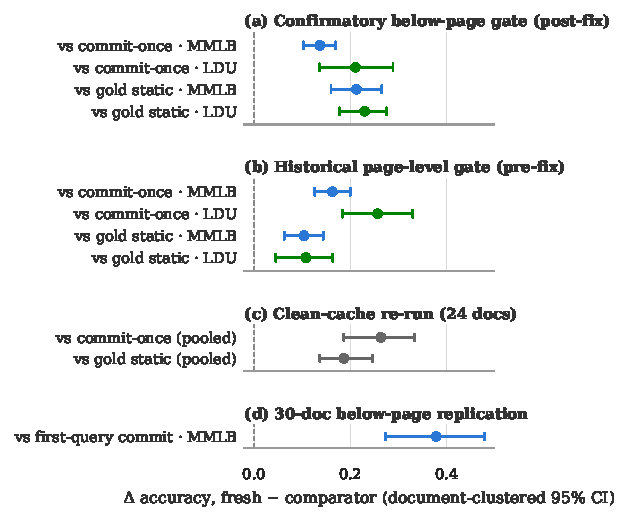
\includegraphics[width=\columnwidth]{figures/fig_reversibility_forest.pdf}
\caption{Document-clustered two-sided 95\% intervals for every executed
isolation contrast (blue MMLB, green LDU, gray pooled over
both cells). \textbf{(a)} The confirmatory below-page gate (\paqc{} as the
fresh arm, full 80-document pins, post-fix code; identical to
Figure~3a). \textbf{(b)} The historical page-level gate
(pre-fix cohort). \textbf{(c)} The clean-cache re-run of
Appendix~\ref{app:integrity}. \textbf{(d)} The 30-document below-page
replication, whose committed arm is the weaker first-query commit
(Appendix~\ref{app:mechanism}). Positive differences favor per-query
re-selection; every interval excludes zero.}
\label{fig:reversibility}
\end{figure}

\paragraph{Decode-identity audit detail.} The six audited document-query
pairs of \S3 span $32$K to $122$K tokens, a stress range
deliberately wider than the evaluation pin. An earlier single greedy-token
divergence traced to the generation loop's mask-independent fast-path
kernel, not to the mask.

\paragraph{Robustness checks behind \S5.1.} First,
an independent extension: because the screen pin is embedded in the
confirmatory pin, we re-ran the statistics on the 50 new documents per cell
only ($n=586$ queries), where fresh over commit-once is $+0.180$
$[+0.124,+0.237]$ and fresh over the static $+0.206$ $[+0.161,+0.249]$
(pooled, equal-cell). Second, granularity and history: the same
two-comparator gate passed at page level on this pin (its pre-fix historical
run: $+0.257$/$+0.163$ over commit-once), and the page-level contrast
survives the clean-cache re-run of Appendix~\ref{app:integrity} ($+0.264$,
$\lb$ $+0.187$), so the effect is not specific to block
granularity or to the fix. Third, scorer generality: the same
fresh-over-stale collapse holds for a retrieval scorer, with ColQwen2 fresh
at $0.423$ versus stale at $0.178$ (historical page-level cohort;
query-micro; equal-cell pooling agrees). The pre-registered
``commitment-pressure'' gradient failed its formal interaction test with
both intervals including zero.

Figure~\ref{fig:reversibility} summarizes the confirmatory below-page gate and its supporting replications. For the confirmatory gate, missingness is a non-issue: all 907 pinned queries completed with zero skips, so the pre-registered adversarial imputation guard (fresh scored $0$, comparators scored $1$ on any incomplete query) never binds. All three arms realize a matched ${\approx}6.0\%$ of context. Supporting analyses from the historical page-level run (pre-fix cohort, labelled): (i) \emph{answerable subset} (secondary, since it conditions on a model outcome): on queries where oracle-evidence scores exactly 1 ($n=407$), fresh $0.583$ vs.\ commit-once $0.182$ ($+0.395$ $[+0.324,+0.460]$) and vs.\ the static $0.382$ ($+0.204$ $[+0.135,+0.266]$); (ii) \emph{budget curves}: the fresh page-level selector dominates both static comparators at every budget in $\{2.5, 5, 10\}\%$ on both cells.

\paragraph{Cache-pollution quantification.} The in-place cache bug of \S4.4 was quantified before being fixed: on a 6-documents-per-cell diagnostic (87 query-rows), the bug inflates gold-page recall by ${\approx}+0.05$ for a fixed scoring head and shifts selections (mean top-$B$ Jaccard clean vs.\ polluted $0.82$, drifting from $1.00$ at $q_0$ to $0.61$ at $q_6$), as expected for cumulative contamination. The recall gate behind the \paqt{} numbers was regenerated clean before any accuracy read (clean held-out expert recall $0.683$/$0.626$ vs.\ polluted $0.674$/$0.628$), and the clean cross-validation picks a more robust head. Absolute fresh-arm accuracy in the pre-fix confirmatory run carries ${\approx}0.04$ inflation (clean $-$ polluted $-0.041$ $[-0.077,-0.003]$ on the 24-document check); the isolation contrasts cancel the bug and stand.

\subsection{Selection Anatomy on MMLB}\label{app:anatomy}
% Source: BASED research/paq_metrics_expansion.json (scripts/paq_metrics_expansion.py,
% BASED commit afd8c7f): artifact-only re-slices of the retained 80-doc dev-pin rows;
% comparator = corrected ColQwen2 loader (cached rf + the 34 corrected re-read values);
% instrument = paq.cluster_lb95 (doc-cluster paired bootstrap, 10k draws, seed 0).

These are descriptive re-slices of the retained per-query development-pin rows (444 decoded / 440 paired, corrected ColQwen2 loader throughout); no pre-frozen bar attaches to them.

\paragraph{Gold-page recall vs.\ accuracy.} At the nominal 5\% budget, two recall notions bracket what each method hands the reader. Coverage-weighted (the fraction of gold-page \emph{tokens} the reader may attend; the budget-comparable notion, since ColQwen2 keeps whole pages): ColQwen2 $0.539$ vs.\ \paqc{} $0.344$, a deficit of $-0.195$ $[-0.236,-0.152]$ for \paqc{}. Any-block-touch (a gold page counts as recalled if any selected 64-token block overlaps it): \paqc{} $0.912$, but this notion flatters block granularity, since \paqc{}'s selections scatter over a median of $10$ pages per query. So the retriever delivers substantially more gold-evidence tokens at matched budget, touches fewer of the right pages, and still loses the accuracy comparison by $+0.077$ (Table~1): recall-optimized selection is not accuracy-optimized selection, consistent with the sharp-scorer negative result (Appendix~\ref{app:negatives}).

\begin{table}[t]
\centering\small
\setlength{\tabcolsep}{1.3pt}%
\begin{tabular}{lrrccc}
\toprule
Stratum & $n$ & docs & \paqc{} & ColQ. & $\Delta$ [95\% CI] \\
\midrule
Chart       & 102 & 35 & 0.409 & 0.311 & $+0.098\,[+0.025,+0.176]$ \\
Figure      & 156 & 53 & 0.393 & 0.333 & $+0.060\,[-0.020,+0.143]$ \\
Layout      &  47 & 32 & 0.490 & 0.338 & $+0.152\,[+0.032,+0.252]$ \\
Pure text   & 144 & 52 & 0.356 & 0.308 & $+0.048\,[-0.010,+0.104]$ \\
Table       & 120 & 38 & 0.353 & 0.258 & $+0.096\,[+0.033,+0.163]$ \\
\midrule
Single-page & 256 & 74 & 0.526 & 0.471 & $+0.054\,[+0.001,+0.108]$ \\
Cross-page  & 184 & 70 & 0.238 & 0.129 & $+0.109\,[+0.052,+0.170]$ \\
\bottomrule
\end{tabular}
\caption{Paired \paqc{}@5\% $-$ ColQwen2-fresh (corrected loader) by MMLB evidence stratum on the 440-query paired cohort (document-cluster paired bootstrap). Evidence-source labels are the benchmark's own and are multi-label (a query counts under each listed source); single- vs.\ cross-page splits on the number of annotated gold pages. The improvement concentrates on cross-page evidence and on chart/table/layout sources; these are descriptive development-pin strata, not pre-registered claims.}
\label{tab:anatomy-strata}
\end{table}

\paragraph{Evidence-type stratification.} Table~\ref{tab:anatomy-strata} stratifies the main paired comparison by the benchmark's evidence annotations. The cross-page stratum roughly doubles the single-page contrast ($+0.109$ vs.\ $+0.054$), and the source strata whose intervals exclude zero (chart, table, layout) are those whose evidence a page-level retriever must fetch whole even when only a small region answers the question.

\subsection{Negative Results}\label{app:negatives}

\paragraph{Per-head mixture transfer gate.} No LoRA adapter was ever trained: this pre-frozen check failed first and stopped that line of work. We fit a logistic per-head mixture over all $36{\times}32=1{,}152$ (layer, head) question-to-page attention channels on off-benchmark provenance-checked data. The transfer gate fails: mixture gold-page recall is $0.652$/$0.594$ vs.\ $0.676$/$0.616$ for the single head, with pooled mixture $-$ single $=-0.023$ $[-0.037,-0.008]$ (907 queries), so the mixture overfits and this direction was closed. The best zero-benchmark-contact head (L21.H18) still coincides with the benchmark-supervised expert layer.

\paragraph{Sharp expert head as block scorer.} Replacing \paqc{}'s diffuse mean-attention block scorer (V0) with the sharp head L21.H18 (V1) fails the pre-frozen gate: on LDU it only nudges the point estimate (from $0.5315$ to $0.536$; V1 $-$ ColQwen2 $= +0.024$ $[-0.012,+0.066]$) and does not separate from V0 (the V1$-$V0 $\lb$ is $-0.011$, n.s.), while on MMLB it hurts (from $0.402$ to $0.381$ on the screen documents). As elsewhere in this study, recall-optimized selection is not accuracy-optimized selection.

\subsection{The Page-Level System in Detail}\label{app:pagelevel}
% RESOLVED 2026-07-26: predecessor material, retained as historical context.
% The confirmatory isolation evidence now comes from the below-page gate
% (\S sec:results-isolation / tab:isolation); this section documents the v1
% page router and its (pre-fix, uncorrected-loader) cohort, labelled as such.

The name \paq{} abbreviates ``Prefill once, Ask many Queries''; unsuffixed \paq{} denotes the earlier page-level router (v1) detailed in this appendix, \paqt{} its expert-head variant, and \paqc{} the below-page KV-mask method of the main text. All numbers in this section are on the 903-query confirmatory cohort (page-level arms), where ColQwen2-fresh scores $0.512$/$0.328$ (LDU/MMLB) with the uncorrected loader; it is distinct from the below-page cohort used in the main comparison (where the corrected-loader ColQwen2-fresh MMLB is $0.3282$, \S4.4). The loader correction is immaterial (\S4.4), so the page-level parity conclusions are unaffected.

\paragraph{The page router (\paq{} v1).} Pages are rendered at coarse resolution (${\approx}3.5$K visual tokens total, i.e.\ ${\approx}70$ tokens/page on a 50-page document) and prefilled once; per query, the question rows' attention (mean over heads, layers, and question tokens) scores pages; the top pages at budget $b$ are re-rendered at full resolution and read. This is page routing rather than KV compression, and it claims no memory savings.

\paragraph{Comparison against trained retrieval.} At $b=5\%$, ColQwen2-fresh scores $0.512$/$0.328$ vs.\ \paq{} $0.386$/$0.258$: pooled $-0.099$ $[-0.129,-0.072]$, a loss of roughly 10 points that holds on every stratum we examined (Figure~\ref{fig:retrieval}). Gold-page recall is consistent with a coverage contribution: ColQwen2-fresh $0.664$/$0.536$ vs.\ \paq{} $0.494$/$0.443$. Both scorers collapse when committed once (ColQwen2 stale $0.216$/$0.138$), reproducing the reversibility pattern with a second scorer family.

% Figure source: scripts/make_fig_pagelevel_reversal_bars.py (values transcribed
% from BASED/research/paq_verdict.json, historical page-level cohort).
\begin{figure}[t]
\centering
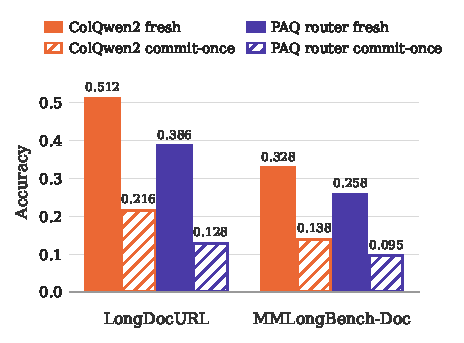
\includegraphics[width=0.95\columnwidth]{figures/fig_pagelevel_reversal_bars.pdf}
\caption{Two observations from the page-level system, per cell (solid bars =
per-query fresh selection, hatched open bars = the same scorer committed
once): (i) ColQwen2-fresh outperforms the page-level attention router (a loss
of roughly 10 points for the router); (ii) \emph{both} scorers collapse when
committed once, so reversibility is a general property of the multi-query
regime rather than being scorer-specific. \paq{} here is the earlier
page-level router of this appendix, not \paqc{}; the below-page \paqc{}
comparison at matched budget is in Table~1. Historical cohort,
uncorrected ColQwen2 loader (disclosed above).}
\label{fig:retrieval}
\end{figure}

\paragraph{\paqt{}: expert-head recall and the parity accuracy evaluation.} Scoring with a single expert (layer, head) chosen by held-out-document cross-validation (CAPS's technique) lifts held-out gold-page recall@5\% to $0.683$ ($n{=}451$) / $0.626$ ($n{=}425$), meeting or exceeding ColQwen2's in-harness $0.664$/$0.536$; mean aggregation at higher scoring resolution moves almost nothing ($0.494/0.443 \to 0.500/0.452$), so the head, not the resolution, is the lever. All selected fold heads sit in layer 21. The pre-registered accuracy evaluation (bars frozen before the run; same reader, render policy, and scorer as the cached baseline rows; only the selected page set differs) lands at parity: \paqt{} $0.518$/$0.357$ vs.\ ColQwen2-fresh $0.512$/$0.328$; deltas $+0.006$ $[-0.018,+0.030]$ and $+0.028$ $[+0.001,+0.055]$; pooled $+0.017$ $[-0.000,+0.035]$. This is non-inferior under the frozen lower-bound margin ($>{-0.03}$) on both cells but not the pre-registered improvement criterion (all lower bounds $>0$), and we do not present the marginal per-cell interval as evidence of superiority. The initially better-looking complete-case verdict (pooled $+0.023$, $\lb$ $+0.005$) was blocked in review for informative missingness: the ${\approx}4\%$ of queries whose high-resolution scoring ran out of memory had cached baseline accuracy $0.62$, far above the cell means; a conservative reduced-resolution recovery of 31/35 missing rows (degrading only the \paqt{} arm, never the baseline) erased the pooled edge. Two caveats carry over: head selection is cross-validated \emph{benchmark-supervised} model selection (not zero-shot; the externally selected L21.H18 of the negative transfer-gate ablation later removed this caveat from the head's existence, though not from its benchmark-tuned use), and the expert-head technique is CAPS's, so the residual novelty at page level is only the amortized one-prefill-many-queries architecture.

\subsection{Systems Measurements in Detail}\label{app:systems}
% Moved here from main-paper \S5.4 (2026-07-29 page-limit pass); every
% number verbatim. The main paper keeps a compressed summary and points to
% "Supplementary Table S10" (= tab:systems below).

We measured the deployment profile of the true \paqc{} path (below-page
masked decode over the \emph{retained} full-document KV cache) against
ColQwen2-fresh and full context on an 8-document, 31-query systems subset of
the pin (single GPU, frozen configuration; Table~\ref{tab:systems}). \paqc{}
is roughly $2.25\times$ slower per online query than the retriever pipeline
and retains a multi-gigabyte per-document cache where the retriever stores a
megabyte-scale page index, but it is roughly $11\times$ faster than
re-reading the document for every question, and the one-time prefill
amortizes after about one query per document. \paqc{} therefore does not
reduce resident KV memory; it trades retained cache state for reversible
query-specific selection. The efficiency claim is simplicity and deployment
shape, not speed: no separately trained retriever checkpoint, no stored
vector index, one deployed model, and no repeated full-document prefills.

\begin{table}[t]
\centering\small
\setlength{\tabcolsep}{4pt}% permitted narrowing (AAAI kit)
\setlength{\tabcolsep}{1.2pt}%
\begin{tabular}{lcccccc}
\toprule
 & extra & per-doc & cold st. & online & amort. & VRAM \\
 & params & state & /doc (s) & /q (s) & /q (s) & (GiB) \\
\midrule
\paqc{} (ours)   & $0$        & $8.15$\,GiB & $11.3$ & $1.04$  & $3.07$  & $44.5$ \\
ColQwen2-fresh   & $2.246$\,B & $11$\,MiB   & $2.5$  & $0.46$  & $0.91$  & $21.8$ \\
full-context     & $0$        & n/a         & n/a    & $11.59$ & $11.59$ & $44.6$ \\
\bottomrule
\end{tabular}
\caption{Deployment profile on an 8-document / 31-query systems subset (frozen configuration, single GPU). ``Extra params'' = additional retriever/selector parameters beyond the shared reader. ``Cold start'' is the one-time per-document cost: full-document prefill for \paqc{}, page-embedding index build for ColQwen2. ``Amort.\ lat./q'' adds the cold start amortized at the development pin's observed $5.55$ queries/document to the online latency (at the systems subset's own $3.9$ queries/document the figures are $3.95$/$1.10$/$11.59$\,s). \paqc{}'s online latency decomposes into $0.19$\,s selection and $0.85$\,s masked decode; it is ${\approx}2.25\times$ slower and far heavier in resident state than ColQwen2, and ${\approx}11\times$ faster than full context (cold start amortized after $N{\approx}1.07$ queries/document). \paqc{}'s online latency excludes ${\approx}1.99$\,s/query of removable research-harness input reconstruction (component sum ${\approx}3.03$\,s/query in the current implementation); mean generated lengths differ across arms ($5.3$/$3.5$/$4.1$ tokens for \paqc{}/ColQwen2/full-context).}
\label{tab:systems}
\end{table}

\section{Additional Limitations Detail}\label{app:limitations-detail}
\paragraph{LDU conversion-bound decomposition.} A re-analysis of the executed rows suggests the shortfall there lies largely past selection: of the 463 rows, ${\approx}39\%$ fail under both \paqc{} and the gold-page oracle (zero even when handed the native-resolution gold pages), only ${\approx}10\%$ are oracle-right/\paqc{}-wrong (the selection-capturable pool), and $2.2\%$ are \paqc{}-right/oracle-wrong, so the oracle is not a strict ceiling; that no selection method can rescue these queries is an observation about this dataset, not a general rule. Native resolution already saturates the prefill on 79/80 documents, and large documents are a flat, low-leverage half. Among pure-selection levers, only a marginal oracle-chooser union passes ($\lb$ $+0.003$; not deployable); only a \paqc{}${\cup}$ColQwen2 hybrid passes comfortably ($\lb$ $+0.061$), and we exclude it as not a standalone method. We therefore offer the dispersed-vs-conversion-bound split as a hypothesis from two datasets.

\paragraph{Base-model ceiling counts.} A large fraction of queries receive no credit even given exactly the annotated gold pages: the oracle-evidence arm scores $0$ on $317/903=35.1\%$ of confirmatory queries and a full $1$ on only $45.1\%$. Pairing controls for shared query difficulty; the oracle is not a strict ceiling (a selected page set can score above the annotated gold set on individual queries).

\paragraph{Remaining protocol caveats.} The commit-once aggregate uses the first $M{=}\min(3,k)$ queries in frozen arrival order (order-permutation and $M$-sensitivity checks remain to be run; the order-free static partially covers this), and the page-level confirmatory run predates the cache fix (\S4.4); its isolation \emph{contrasts} were verified robust, but its absolute fresh-arm levels carry ${\approx}0.04$ inflation on the 24-document check.

\bibliography{references,references_extbench}

\end{document}
